% Author: Jørn Olav Jensen

\newpage
\section{Suggested solutions: Time-frequency Uncertainty Principle}

\begin{enumerate}
  % Exercise 1
  \item The Hann window in continuous-time is defined as:
        \[ h_{1}(t)=\begin{cases}
            \sin^{2}(\pi t/T), \quad 0\le t\le T, \\
            0, \quad \text{otherwise}.
          \end{cases} \]
        Define the length of the Hann filter to be $T$ in time-domain.
        The Fourier transform of $h_{1}(t)$ can be shown to be:
        \[ \mathcal{H}_{1}(\omega)=\left[\frac{\sin(\frac{T}{2}\omega)}{\omega}+\frac{1}{2}\frac{\sin(\pi-\frac{T}{2}\omega)}{\frac{2\pi}{T}-\omega}+\frac{1}{2}\frac{\sin(\pi+\frac{T}{2}\omega)}{\frac{2\pi}{T}+\omega}\right]e^{-i\frac{T}{2}\omega}. \]
        Let $h_{2}(t)$ denote the rectangular window of length $T$, for which the Fourier transform is:
        \[ \mathcal{H}_{2}(\omega)=\frac{2\sin(\frac{T}{2}\omega)}{\omega}e^{-i\frac{T}{2}\omega}, \]
        which also has length taken to be $T$.

        \begin{enumerate}[a)]
          % Exercise 1a)
          \item Using the Fourier transform we have:
                \begin{align*}
                  \mathcal{H}_{1}(\omega) & =\int_{-\infty}^{\infty}\sin^{2}(\pi t/T)e^{-i\omega t}dt=\frac{1}{(2i)^{2}}\int_{0}^{T}\left(e^{i \pi t/T}-e^{-i\pi t/T}\right)^{2}e^{-i\omega t}dt, \\
                                          & =-\frac{1}{4}\int_{0}^{T}\left[e^{-i(\omega -2\pi/T)t}-2e^{-i\omega t}+e^{-i(\omega + 2\pi/T)t}\right]dt.                                             \\
                \end{align*}
                Last handle each term on its own, the first term is computed as:
                \begin{align*}
                  \int_{0}^{T}e^{-i(\omega-2\pi/T)t}dt & =\left[-\frac{1}{i(\omega-\frac{2\pi}{T})}e^{-i(\omega-2\pi/T)t}\right]_{0}^{T}=\frac{1}{i(\omega-\frac{2\pi}{T})}(1-e^{-i(\omega T-2\pi)}), \\
                                                       & =\frac{1}{i(\omega-\frac{2\pi}{T})}(e^{i(\omega T/2-\pi)}-e^{-i(\omega T/2-\pi)})e^{-i(\omega T/2-\pi)},                                     \\
                                                       & =\frac{2}{\omega-\frac{2\pi}{T}}\sin\left(\omega\frac{T}{2}-\pi\right)e^{-i\omega\frac{T}{2}}\overbrace{e^{i\pi}}^{-1},                      \\
                                                       & =-\frac{2}{\frac{2\pi}{T}-\omega}\sin\left(-\left(\pi-\omega\frac{T}{2}\right)\right)e^{-i\omega\frac{T}{2}}(-1),                            \\
                                                       & =-\frac{2}{\frac{2\pi}{T}-\omega}\sin\left(\pi-\omega\frac{T}{2}\right)e^{-i\omega\frac{T}{2}},
                \end{align*}
                the last step uses $\sin(-\theta)=-\sin(\theta)$. The second term is:
                \begin{align*}
                  \int_{0}^{T}e^{-i\omega t}dt & =\left[-\frac{1}{i\omega}e^{-i\omega t}\right]_{0}^{T}=\frac{1}{i\omega}(1-e^{-i\omega T}),                                                      \\
                                               & =\frac{1}{i\omega}(e^{i\omega T/2}-e^{-i\omega T/2})e^{-i\omega T/2}=\frac{2}{\omega}\sin\left(\omega\frac{T }{2}\right)e^{-i\omega\frac{T}{2}},
                \end{align*}
                and finally, the same approach as the first gives:
                \begin{align*}
                  \int_{0}^{T}e^{-i(\omega+2\pi/T)t}dt & =\left[-\frac{1}{i(\omega+\frac{2\pi}{T})}e^{-i(\omega+2\pi/T)t}\right]_{0}^{T}=\frac{1}{i(\omega+\frac{2\pi}{T})}(1-e^{-i(\omega T + 2\pi)}), \\
                                                       & =\frac{1}{i(\omega+\frac{2\pi}{T})}(e^{i(\omega T/2+\pi)}-e^{-i(\omega T/2+\pi)})e^{-i(\omega T/2+\pi)},                                       \\
                                                       & =\frac{2}{\omega+\frac{2\pi}{T}}\sin\left(\omega\frac{T}{2}+\pi\right)e^{-i\omega\frac{T}{2}}\overbrace{e^{-i\pi}}^{-1},                       \\
                                                       & =-\frac{2}{\frac{2\pi}{T}+\omega}\sin\left(\pi+\omega\frac{T}{2}\right)e^{-i\omega\frac{T}{2}}.
                \end{align*}
                Putting everything together with the correct signs and factors we obtain:
                \[ \mathcal{H}_{1}(\omega)=\left[\frac{\sin\left(\omega\frac{T }{2}\right)}{\omega}+\frac{1}{2}\frac{\sin\left(\pi-\omega\frac{T}{2}\right)}{\frac{2\pi}{T}-\omega}+\frac{1}{2}\frac{\sin\left(\pi+\omega\frac{T}{2}\right)}{\frac{2\pi}{T}+\omega}\right]e^{-i\frac{T}{2}\omega} \]
                as desired.

          % Exercise 1b)
          \item If the peak of the Hann window is at $t=T/2$, then we can shift the peak to be at $t=0$ as follows:
                \[ h(t)=h_{1}\left(t-\frac{T}{2}\right)=\sin^{2}\left(\frac{\pi}{T}\left(t-\frac{T}{2}\right)\right)=\sin^{2}\left(\frac{\pi}{T}t-\frac{\pi}{2}\right)=\cos^{2}\left(\frac{\pi}{T}t\right), \]
                as $\sin\left(\theta-\frac{\pi}{2}\right)=-\cos(\theta)$.

          % Exercise 1c)
          \item To plot the spectral responses, we can use Listing \ref{code14_1}.
                \lstinputlisting[language=Python, caption=Filter spectral response, label=code14_1, linerange={0-27}]{ch14/code/ex14_1.py}

                The magnitude response is shown in Figure \ref{ex:filters}. The Figure shows that the Hann window manages the
                rejection of frequencies out of the band-pass better than the rectangular window.
                \begin{marginfigure}
                  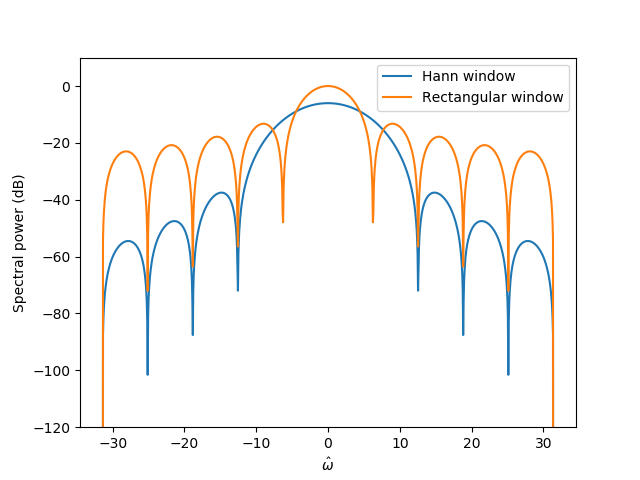
\includegraphics[width=7.0cm,height=7.5cm]{ch14/figures/filters.png}
                  \caption{Comparison of the spectral responses of two filters}
                  \label{ex:filters}
                \end{marginfigure}

          % Exercise 1d)
          \item By inspecting Figure \ref{fig:hann_ct_ex_mr} we conclude that the rectangular window (in red)
                has its first zero at $\omega=\omega_{2}$, while the Hann window (in blue) has the first zero at $\omega=\omega_{1}$.
                By investigating the plot it appears that $\omega_{1}=2\omega_{2}$, where $\omega_{2}=2\pi /T$ as given.
                The width of the rectangular window is then $\Delta\omega_{2}=2\omega_{2}=4\pi/T$, meaning that the
                width of the Hann window is $\Delta\omega_{1}=2\omega_{1}=2(4\pi/T)=2\Delta\omega_{2}=8\pi /T$.

          % Exercise 1e)
          \item We've shown that:
                \begin{align*}
                  \Delta\omega_{1} & =4\pi/T, \\
                  \Delta\omega_{2} & =8\pi/T,
                \end{align*}
                so the rectangular window needs to be $T=2$ seconds long, while the Hann window needs to be $T=4$ seconds long.

          % Exercise 1f)
          \item By Figure \ref{fig:hann_ct_ex_mr}: the Hann window cuts the power to approximately $-60\ \text{dB}$,
                which is around $10^{-6}$, while the rectangular window only cuts around $-20\ \text{dB}$ 
                which corresponds to $10^{-2}$, so not that much reduction. The Hann window does a far better 
                job in reducing the edges than the rectangular window.

          % Exercise 1g)
          \item As discussed in f) the Hann window is much better at handling frequencies outside the band-pass.
                This can be seen from the plot of the power of the magnitude response. Thus, the Hann window 
                can be used much more efficiently to reduce spectral leakage which in many cases can 
                be a huge problem, so the trade-off when comparing filter width to spectral leakage, 
                reducing the leakage is preferred over reducing the filter width.
        \end{enumerate}

  % Exercise 2
  \item Let $\Psi(x)$ be given as:
        \begin{equation*}
          \Psi(x) = \frac{1}{\sqrt{2T}}[u(x + T) - u(x - T)].
        \end{equation*}

        \begin{enumerate}[a)]
          % Exercise 2a)
          \item Using the unitary Fourier transform, we can directly compute it as:
                \begin{align*}
                  \hat{\Psi}(k) & = \frac{1}{\sqrt{2\pi}}\int_{-\infty}^{\infty}\Psi(x)e^{-ik x}dx,                         \\
                                & = \frac{1}{\sqrt{2\pi}\sqrt{2T}}\int_{-\infty}^{\infty} [u(x + T) - u(x - T)]e^{-ik x}dx, \\
                                & = \frac{1}{\sqrt{4\pi T}}\int_{-T}^{T}e^{-ik x}dx,                                        \\
                                & = \frac{1}{2ik\sqrt{\pi T}}[e^{ik T} - e^{-ik T}],                                        \\
                                & = \frac{1}{\sqrt{T\pi}}\frac{\sin(k T)}{k},
                \end{align*}
                where we've used that $\sin\theta = \frac{1}{2i}(e^{i\theta}-e^{-i\theta})$.

          % Exercise 2b)
          \item Have that:
                \begin{align*}
                  |\Psi(x)|^{2}       & = \frac{1}{2T}[u(x+T) - u(x-T)],             \\
                  |\hat{\Psi}(k)|^{2} & = \frac{1}{T\pi}\frac{\sin^{2}(k T)}{k^{2}}.
                \end{align*}
                For $|\Psi(x)|^{2}$, we see that $\Delta x = T$ and for $|\hat{\Psi}(k)|^{2}$, 
                we get $\Delta k =\pi/T$. The time-frequency uncertainty can then be expressed as
                \[ \Delta x\Delta k=(T)\left(\frac{\pi}{T}\right)=\pi. \]

          % Exercise 2c)
          \item The wave functions $\Psi(x)$ and $\hat{\Psi}(k)$ are shown in Figure \ref{x:wavefunction} 
                and Figure \ref{k:wavefunction}, respectively.
                \begin{marginfigure}
                  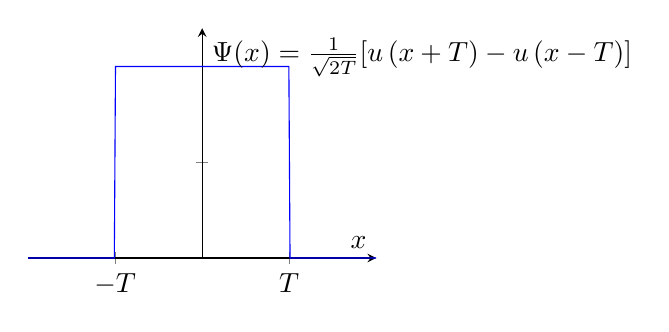
\begin{tikzpicture}
                    \begin{axis}[domain=(-1):(1),samples=300,
                        width=6cm,
                        height=4.5cm,
                        ymin=0,ymax=1.2,
                        xlabel={$x$},
                        ylabel={$\Psi(x)=\frac{1}{\sqrt{2T}}[u\left(x+T\right) - u\left(x-T\right)$]},
                        axis x line=center,
                        axis y line=center,
                        yticklabels={,,,},
                        xtick={-0.5,0.5},
                        xticklabels={$-T$,$T$}
                      ]

                      \addplot[blue] {(x>-0.5)*(x<0.5)};
                    \end{axis}
                  \end{tikzpicture}
                  \caption{The wave function $\Psi(x)$ in position space, with $\Delta x=T$.}
                  \label{x:wavefunction}
                \end{marginfigure}

                \begin{marginfigure}
                  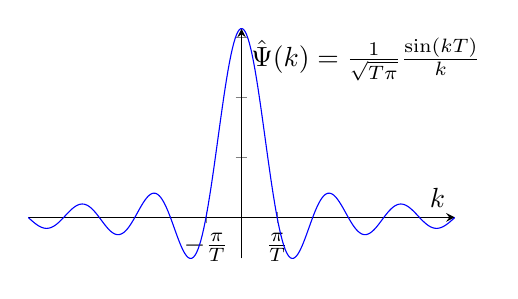
\begin{tikzpicture}
                    \begin{axis}[domain=(-6):(6),samples=300,
                        width=7cm,
                        height=4.5cm,
                        xlabel={$k$},
                        ylabel={$\hat{\Psi}(k)=\frac{1}{\sqrt{T\pi}}\frac{\sin(k T)}{k}$},
                        axis x line=center,
                        axis y line=center,
                        yticklabels={,,,},
                        xtick={-1.0,1.0},
                        xticklabels={$-\frac{\pi}{T}$,$\frac{\pi}{T}$}
                      ]
                      \addplot[blue] {sin(deg(3.14 * x))/x};
                    \end{axis}
                  \end{tikzpicture}
                  \caption{The wave function $\hat{\Psi}(k)(k)$ in wavenumber space, with $\Delta k=\frac{\pi}{T}$.}
                  \label{k:wavefunction}
                \end{marginfigure}

          % Exercise 2d)
          \item By Parseval's theorem, we have, in the unitary case:
                \[ \int_{-\infty}^{\infty} |x(t)|^{2}dt=\int_{-\infty}^{\infty}|\hat{x}(\omega)|^{2}d\omega. \]
                Using this, we get:
                \begin{align*}
                  \int_{-\infty}^{\infty}|\Psi(x)|^{2}dx & =\int_{-\infty}^{\infty}\frac{1}{2T}[u(x + T) - u(x - T)]dx, \\
                                                         & = \frac{1}{2T}\int_{-T}^{T}dx=1,
                \end{align*}
                thus, by the unitary form of Parseval's theorem, we get:
                \[ \int_{-\infty}^{\infty}|\hat{\Psi}(k)|^{2}dk=\int_{-\infty}^{\infty}|\Psi(x)|^{2}dx=1. \]

          % Exercise 2e)
          \item If the wavefunction for position is given as $\delta(x - x_0)$, then the wavefunction for the wavenumber (or momentum)
                is given by the unitary Fourier transform as:
                \[ \hat{\Psi}(k) = \frac{1}{\sqrt{2\pi}}\int_{-\infty}^{\infty}\delta(x - x_0)e^{-ik x}dx=\frac{1}{\sqrt{2\pi}}e^{-ikx_{0}}. \]
                Then the modulus of the wavefunction is proportional to the probability distribution for the wavenumber, so that:
                \[ |\hat{\Psi}(k)|^{2}=\frac{1}{\sqrt{2\pi}}e^{-ikx_0}\frac{1}{\sqrt{2\pi}}e^{ikx_0}=\frac{1}{2\pi}. \]
                This shows that all wavenumbers are equally likely, so no, we cannot say that 
                any wavenumber/momentum is more probable than any other.

        \end{enumerate}
\end{enumerate}